% !TEX program = lualatex
% Generated by new_homework.sh — Math 118 Homework 4
\documentclass[11pt]{article}

\usepackage{fontspec}
\usepackage{microtype}
\usepackage{mathtools,amssymb,amsfonts,amsthm,bm}
\usepackage{enumitem}
\usepackage{booktabs,array,xcolor}
\usepackage{geometry,fancyhdr,setspace}
\usepackage{pdfpages}
\usepackage{graphicx}
\usepackage[hidelinks]{hyperref}
\usepackage[nameinlink,noabbrev]{cleveref}

% ---------- Page and paragraph rhythm (matches lecture/solutions templates) ----------
\geometry{margin=1in,headheight=15pt}
\setstretch{1.12}
\setlength{\parindent}{0pt}
\setlength{\parskip}{0.55em plus 0.12em minus 0.08em}
\setlength{\abovedisplayskip}{0.8em plus 0.2em minus 0.1em}
\setlength{\belowdisplayskip}{0.8em plus 0.2em minus 0.1em}
\allowdisplaybreaks[3]
\setlist{leftmargin=*,topsep=0.35em,itemsep=0.15em,parsep=0pt}

% ---------- Metadata ----------
\newcommand{\studentname}{Keshav Ramamurthy}
\newcommand{\coursename}{Math 118}
\newcommand{\courselongname}{Fourier Analysis}
\newcommand{\assignment}{Homework 4}
\newcommand{\term}{Fall 2026}

% ---------- Core notation (same as ~/.config/nvim/textemplate.tex) ----------
\newcommand{\N}{\mathbb{N}}
\newcommand{\Z}{\mathbb{Z}}
\newcommand{\Q}{\mathbb{Q}}
\newcommand{\R}{\mathbb{R}}
\newcommand{\C}{\mathbb{C}}
\newcommand{\F}{\mathbb{F}}
\newcommand{\K}{\mathbb{K}}
\newcommand{\E}{\mathbb{E}}
\newcommand{\Prob}{\mathbb{P}}
\newcommand{\1}{\mathbf{1}}
\newcommand{\eps}{\varepsilon}
\newcommand{\dd}{\,\mathrm{d}}
\newcommand{\abs}[1]{\left\lvert#1\right\rvert}
\newcommand{\norm}[1]{\left\lVert#1\right\rVert}
\newcommand{\ip}[2]{\left\langle#1,#2\right\rangle}
\newcommand{\set}[1]{\left\{#1\right\}}
\newcommand{\ceil}[1]{\left\lceil#1\right\rceil}
\newcommand{\floor}[1]{\left\lfloor#1\right\rfloor}
\newcommand{\given}{\,\middle\vert\,}
\newcommand{\indep}{\perp\!\!\!\perp}
\newcommand{\wh}[1]{\widehat{#1}}
\newcommand{\deriv}[2]{\frac{\mathrm{d}#1}{\mathrm{d}#2}}
\newcommand{\pderiv}[2]{\frac{\partial#1}{\partial#2}}
\newcommand{\lto}{\longrightarrow}
\newcommand{\st}{\text{ such that }}
\DeclareMathOperator{\Aut}{Aut}
\DeclareMathOperator{\End}{End}
\DeclareMathOperator{\Gal}{Gal}
\DeclareMathOperator{\Hom}{Hom}
\DeclareMathOperator{\Ker}{ker}
\DeclareMathOperator{\im}{im}
\DeclareMathOperator{\rank}{rank}
\DeclareMathOperator{\nullity}{nullity}
\DeclareMathOperator{\Span}{span}
\DeclareMathOperator{\tr}{tr}
\DeclareMathOperator{\diag}{diag}
\DeclareMathOperator{\spec}{spec}
\DeclareMathOperator{\ord}{ord}
\DeclareMathOperator{\supp}{supp}
\DeclareMathOperator{\diam}{diam}
\DeclareMathOperator{\Var}{Var}
\DeclareMathOperator{\Cov}{Cov}
\DeclareMathOperator*{\argmin}{arg\,min}
\DeclareMathOperator*{\argmax}{arg\,max}

% ---------- Statement environments ----------
\newtheorem{problem}{Problem}
\newtheorem{theorem}{Theorem}
\newtheorem{lemma}{Lemma}
\newtheorem{proposition}{Proposition}
\newtheorem{corollary}{Corollary}
\theoremstyle{definition}
\newtheorem{definition}{Definition}
\newtheorem{example}{Example}
\newtheorem{remark}{Remark}

% ---------- Solution machinery (matches solutions.tex / textemplate.tex) ----------
\newenvironment{solution}{\begin{proof}[Solution]}{\end{proof}}
\newenvironment{answer}{\begin{proof}[Answer]}{\end{proof}}
\renewcommand{\qedsymbol}{\(\square\)}
\newcommand{\exercise}[1]{%
  \par\goodbreak\medskip\noindent\textbf{Exercise #1}\par\nopagebreak\smallskip\nopagebreak}
\newcommand{\exref}[1]{\textsf{\textbf{Exercise~#1}}}
\newenvironment{claim}{\par\smallskip\noindent\textit{Claim.}\ }{\par\smallskip}
\newenvironment{idea}{\par\smallskip\noindent\textit{Idea.}\ }{\par\smallskip}
\newenvironment{proofsketch}{\par\smallskip\noindent\textit{Proof sketch.}\ }{\par\smallskip}

% ---------- Header ----------
\pagestyle{fancy}
\fancyhf{}
\fancyhead[L]{\coursename}
\fancyhead[C]{\assignment\ — my solutions}
\fancyhead[R]{\studentname}
\fancyfoot[C]{\thepage}

\begin{document}

% ---------- Title ----------
\begin{center}
  {\Large\sffamily\bfseries \coursename\ -- \courselongname}\par\vspace{3pt}
  {\sffamily \assignment\ — my solutions}\par\vspace{3pt}
  {\small\sffamily \term\quad\textbullet\quad \studentname}
\end{center}
\medskip
\hrule
\bigskip

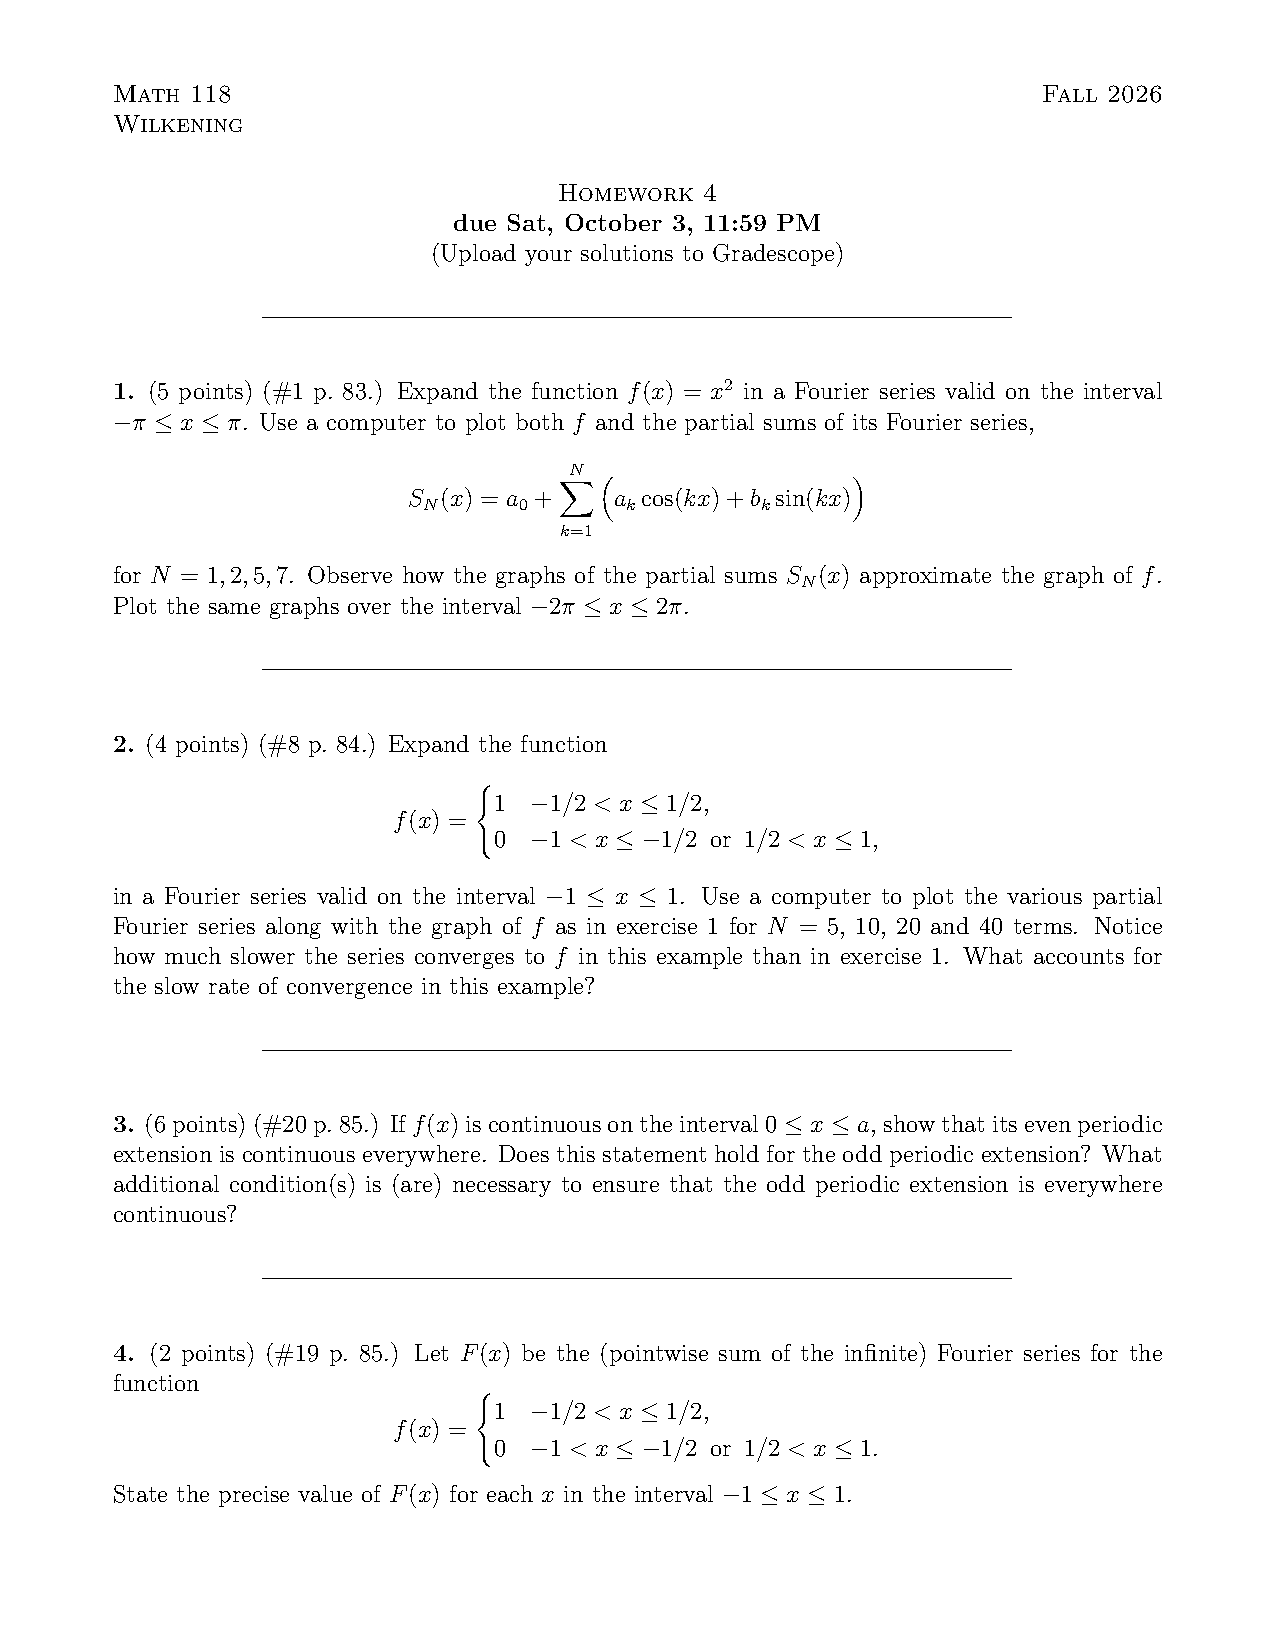
\includepdf[pages=-,pagecommand={\thispagestyle{empty}}]{hw04.pdf}
\clearpage


\section*{Solutions}
\subsubsection*{Problem 1}
\begin{solution}
We start with $f(x)=x^2$. Since it is even, $b_k=0$. The constant term is
\[
a_0=\frac{1}{2\pi}\int_{-\pi}^{\pi}x^2\,dx
=\frac{\pi^2}{3}.
\]
\par For $k\geq1$, since it's even we have
\[
a_k=\frac{2}{\pi}\int_0^\pi x^2\cos(kx)\,dx.
\]
Integrating by parts,
\[
\int_0^\pi x^2\cos(kx)\,dx
=-\frac{2}{k}\int_0^\pi x\sin(kx)\,dx
=\frac{2\pi(-1)^k}{k^2},
\]
so we have that $a_k=4(-1)^k/k^2$. Thus
\[
S_N(x)=\frac{\pi^2}{3}
+4\sum_{k=1}^{N}\frac{(-1)^k}{k^2}\cos(kx).
\]
\par For $N=1,2,5,7$, the partial sums approach $x^2$ on $[-\pi,\pi]$.
\begin{center}
  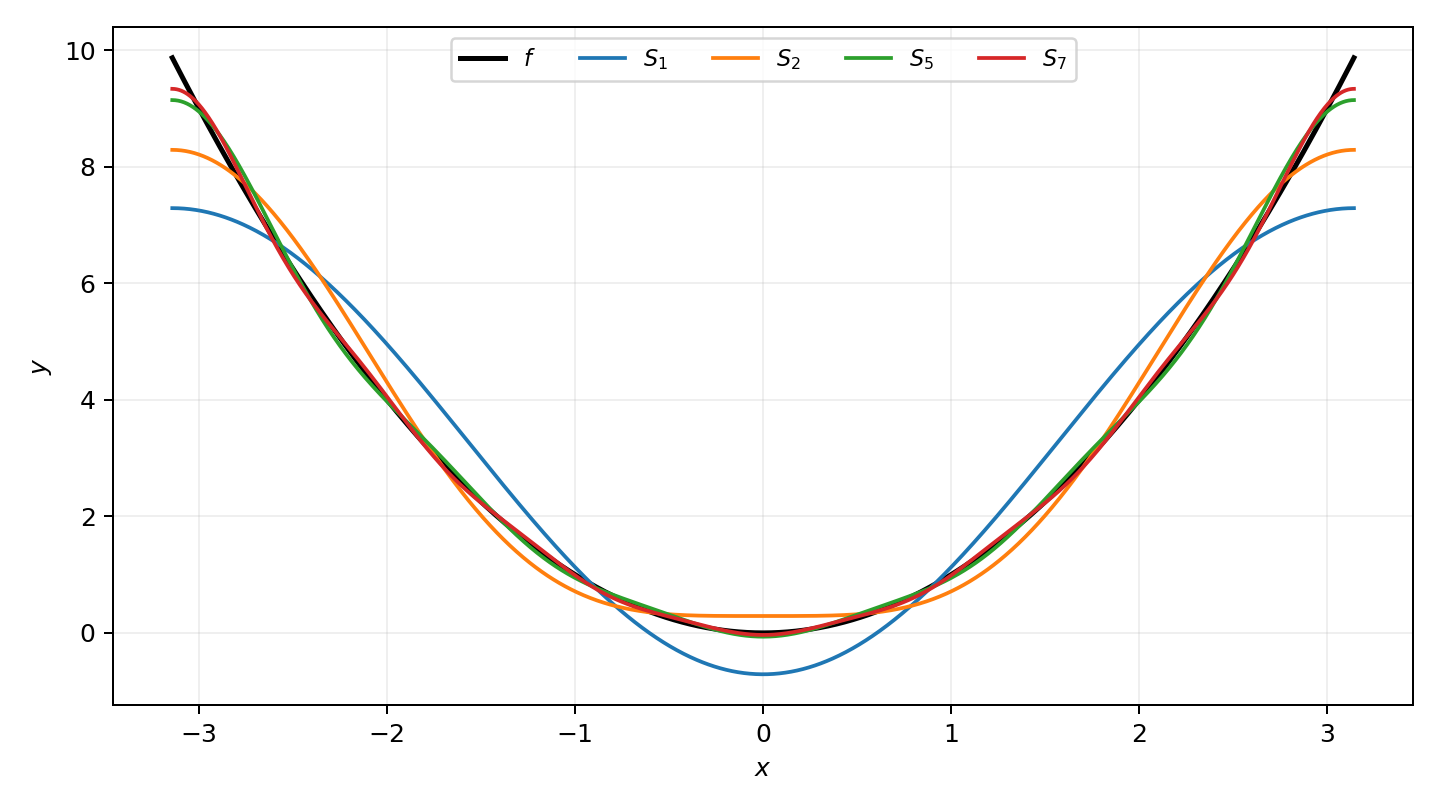
\includegraphics[width=0.95\linewidth]{hw04_problem1_plot.png}
\end{center}
\par Over $[-2\pi,2\pi]$, the series repeats the graph from $[-\pi,\pi]$.
\begin{center}
  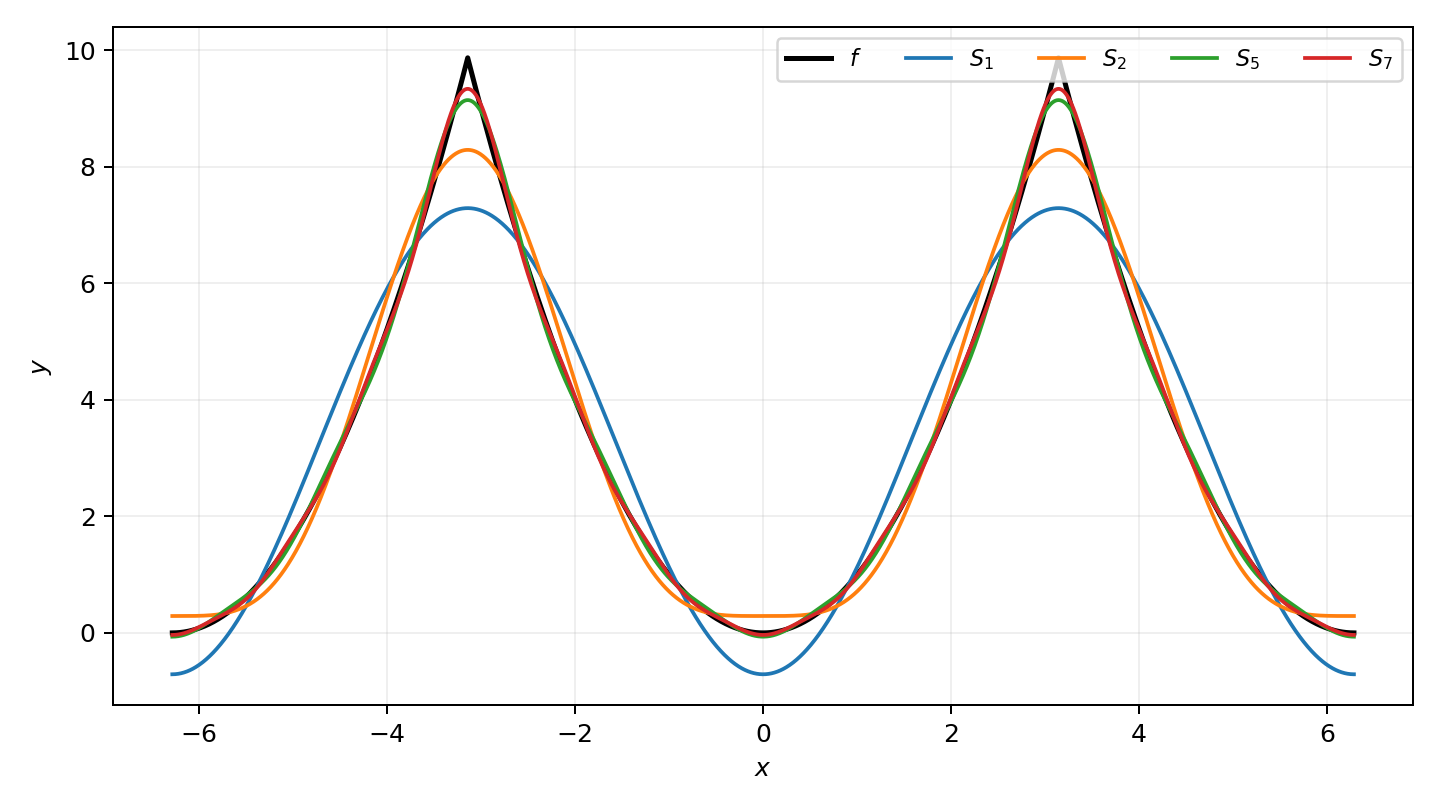
\includegraphics[width=0.95\linewidth]{hw04_problem1_periodic_plot.png}
\end{center}
\end{solution}
\subsubsection*{Problem 2}
\begin{solution}
On $[-1,1]$ the frequencies are $k\pi$, and Since $f$ is even, $b_k=0$, so
the constant term is
\[
a_0=\frac12\int_{-1}^{1}f(x)\,dx
=\frac12\int_{-1/2}^{1/2}1\,dx=\frac12.
\]
\par For $k\geq1$ we have that 
\[
a_k=\int_{-1}^{1}f(x)\cos(k\pi x)\,dx
=\int_{-1/2}^{1/2}\cos(k\pi x)\,dx
=\frac{2\sin(k\pi/2)}{k\pi}.
\]
\par Plugging these back in, we have
\[
F(x)=\frac12+\frac2\pi\sum_{k=1}^{\infty}
\frac{\sin(k\pi/2)}{k}\cos(k\pi x),\qquad
S_N(x)=\frac12+\frac2\pi\sum_{k=1}^{N}
\frac{\sin(k\pi/2)}{k}\cos(k\pi x).
\]
Only odd values of $k$ appear, since $\sin(k\pi/2)=0$ for even $k$.
\par The graph jumps from $0$ to $1$ at $-1/2$ and back to $0$ at $1/2$.
\par The partial sums overshoot near those points, and the nonzero coefficients have factor $1/k$, rather than
$1/k^2$ as in Problem 1, so this series converges more slowly.
\begin{center}
  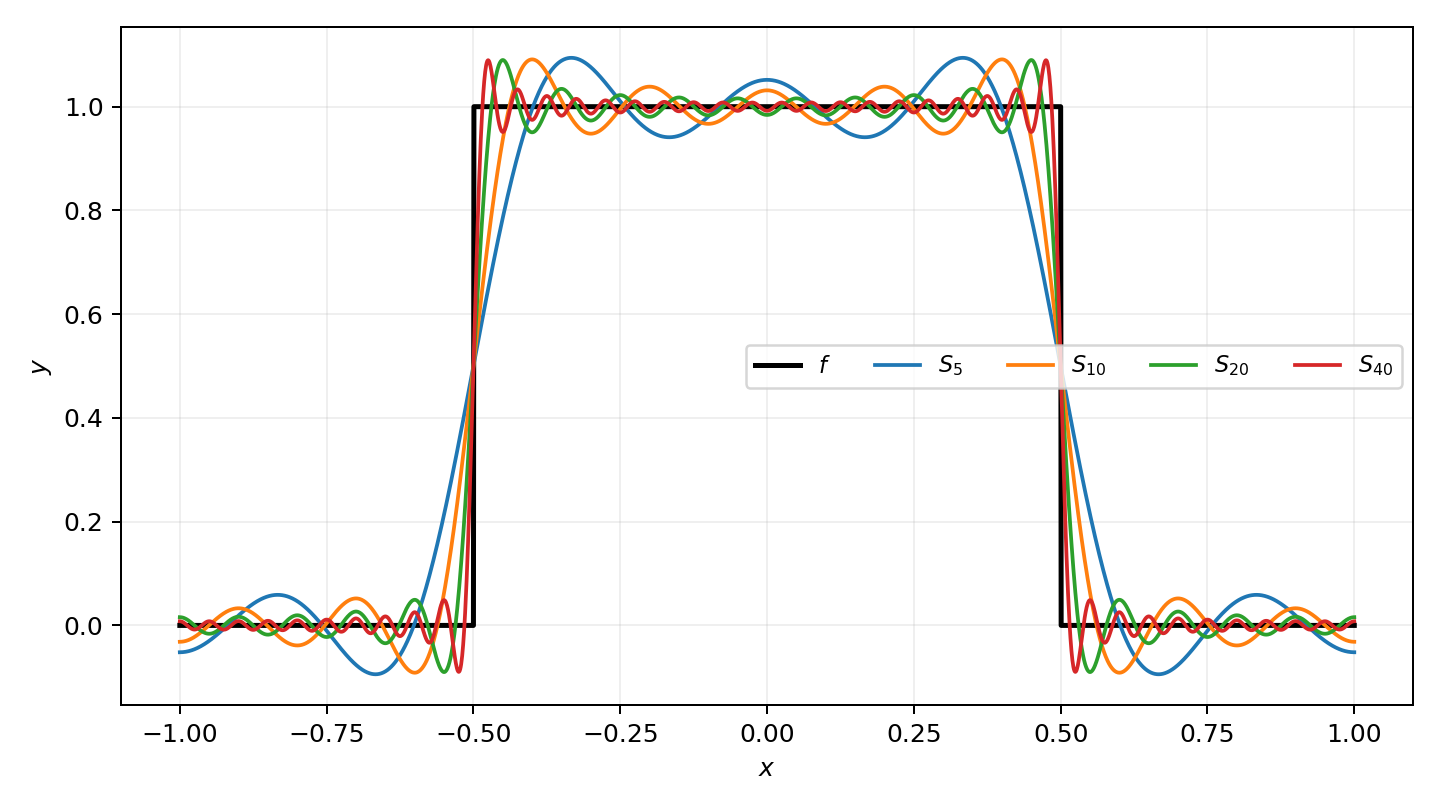
\includegraphics[width=0.95\linewidth]{hw04_problem2_plot.png}
\end{center}
\end{solution}
\subsubsection*{Problem 3}
\begin{solution}
For the even extension, we reflect $f$ across $0$ and repeat every $2a$.
\par The only possible breaks are at $0$ or the endpoints where two meet.
At $0$, both sides go to $f(0)$ and at $-a$ and $a$, they both go to $f(a)$.
\par For any other point where two points meet it is analogous to the endpoints at $-a$ and
$a$ and thus the even extension is
continuous.
\par For the odd extension, the reflected half is $-f(-x)$. The two
limits at $0$ are $-f(0)$ and $f(0)$, and the limits at the ends of
a period are $-f(a)$ and $f(a)$. 
\par Each pair only has equal values exactly when
$f(0)=f(a)=0$, and thus continuity only occurs when $f(0) = f(a) = 0.$
\end{solution}
\subsubsection*{Problem 4}
\begin{solution}
The only jumps are at $x=\pm1/2$. Besides them, 
the fourier series converges to $1$ in the middle interval and $0$ on
the outer intervals. At $x=\pm1$, it also converges to $0$, since the
adjacent periods meet at $0$.
\par At each jump, the left and right values are $0$ and $1$ in some
order. Their average is $\frac{0+1}{2} =\frac{1}{2}$, so
\[
F(x)=
\begin{cases}
1, & -\frac12<x<\frac12,\\[3pt]
\frac12, & x=-\frac12\text{ or }x=\frac12,\\[3pt]
0, & -1\leq x<-\frac12\text{ or }\frac12<x\leq1.
\end{cases}
\]
\end{solution}
\subsubsection*{Problem 5}
\begin{solution}
From Problem 1, the partial sums are
\[
S_N(x)=\frac{\pi^2}{3}
+4\sum_{k=1}^{N}\frac{(-1)^k}{k^2}\cos(kx).
\]
The values at $-\pi$ and $\pi$ are both $\pi^2$, so the repeated pieces
meet at the same value. Each piece is a quadratic, and there are no
jumps where they meet. The Fourier series therefore converges to $x^2$
at every point of $[-\pi,\pi]$, including the endpoints.
\par Since $|\cos(kx)|\leq1$, the size of the tail after $S_N$ is bounded for every
$x$ by
\[
4\sum_{k=N+1}^{\infty}\frac{1}{k^2}.
\]
This tends to $0$ as $N\rightarrow\infty$, so the convergence is
uniform on $[-\pi,\pi]$.
\par Now set $x=\pi$. Since $\cos(k\pi)=(-1)^k$, each term in the
sum is positive. Taking the limit gives
\[
\pi^2=\frac{\pi^2}{3}+4\sum_{k=1}^{\infty}\frac1{k^2}
\quad\rightarrow\quad
\sum_{k=1}^{\infty}\frac1{k^2}=\frac{\pi^2}{6}.\qedhere
\]
\end{solution}

\end{document}
